\addcontentsline{toc}{section}{Приложение Б (Справочное) Статья для Интернет-конференции ГПО}
\begin{center}
Приложение Б\\
(Справочное)\\
Статья для Интернет-конференции ГПО
\end{center}
\vspace{\baselineskip}

\begin{center}
\textbf{ИЗУЧЕНИЕ УЯЗВИМОСТЕЙ ПАМЯТИ И РАЗРАБОТКА КУРСА ЛЕКЦИЙ И ПРАКТИЧЕСКИХ ЗАНЯТИЙ ПО ДИСЦИПЛИНЕ <<ТЕХНОЛОГИИ И МЕТОДЫ ПРОГРАММИРОВАНИЯ>>}\\
\textbf{\textit{Е.И. Косенко, студент, Д.Г. Дудкин, студент каф. КИБЭВС}}\\
\textit{Научный руководитель Д.С.Никифоров, младший научный сотрудник каф. КИБЭВС, Томск, ТУСУР, nds@csp.tusur.ru}\\
\textbf{\textit{Проект ГПО КИБЭВС-1808 Разработка и развитие системы для обучения и проведения практик по информационной безопасности}}\\  
\end{center}
В данной статье рассматривается одна из наиболее распространенных уязвимостей -- переполнение буфера, а также пример кода, предназначенный для демонстрации студентам опасности эксплуатации этой уязвимости в рамках курса <<Технологии и методы программирования>> (ТиМП).\par
\textbf{Ключевые слова:} уязвимость, память, переполнение буфера.\par
\textbf{Введение.} Под термином <<уязвимость>> понимается недостаток в компьютерной системе, эксплуатация которой приводит к нарушению целостности или некорректной работе системы. Такие недостатки были обнаружены во всех основных операционных системах, включая Microsoft Windows, MacOS, а также UNIX.\par 
Проблема переполнения буфера выходит за рамки обычного нарушения целостности или логики функционирования программы и даже может являться причиной удаленного вторжения в систему с прямым наследованием всех привилегий. Данная уязвимость является самой опасной с точки зрения поставщиков ОС и одной из самых значимых в компьютерной безопасности в целом [1].\par 
Актуальность данной проблемы подтверждает тот факт, что уязвимости, относящиеся к переполнению различных сегментов памяти, обнаруживаются специалистами регулярно. Проиллюстрировать этот довод могут две уязвимости, включенные в реестр CVE (common vulnerabilities and exposures -- список общих уязвимостей, подверженных воздействиям извне) за последнее время, а именно CVE-2015-7547 [2] и CVE-2018-10731 [3].\par
Новизна подхода заключается в том, что текущий курс ТиМП не охватывает проблему, описанную выше, и нуждается в развитии и частичной доработке.\par
В ходе работы в рамках ГПО проводится изучение уязвимостей, возникающих при работе с памятью, формирование материалов для проведения занятий по дисциплине ТиМП и подготовка контента для интернет-ресурса freehackquest.com.\par
\textbf{Описание уязвимости <<buffer overflow>>.} Ее смысл заключается в перезаписи данных за пределами стека при переполнении буфера. Рассмотрим данную уязвимость на примере разбора задания <<Smash the stack -- level 3>>, код которого представлен на рисунке 1 [4]. Допустим, злоумышленнику интересен некий абстрактный флаг, скрытый в программе в функции good. Суть экслойта (программы или кода, использующего уязвимость с целью извлечения выгоды) заключается в том, что при передаче в буфер более 50 символов произойдет его переполнение и часть данных перезапишется поверх адреса функции bad.\par 
Таким образом, возникает возможность изменить адрес функции, и, когда код продолжит свое исполнение, в месте предполагаемого вызова функции bad будет вызвана функция good, следовательно злоумышленник получит доступ к секретным данным.\par
\begin{center}
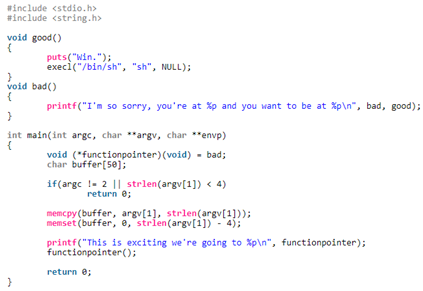
\includegraphics[width=0.65\textwidth]{st1}\\
\small{Рис. 1 -- Код, реализующий переполнение буфера}\\
\end{center}
\vspace{\baselineskip}
Чтобы наглядно продемонстрировать расположение функций и их аргументов в адресном пространстве памяти, код программы был дизассемблирован посредством отладчика GDB. Далее на основе полученных данных было составлено схематическое расположение функций и их аргументов по конкретным адресам в различных сегментах памяти на протяжении всего времени работы программы.\par 
Результаты исследования позволяют <<изнутри>> понять, что происходит в памяти компьютера после запуска программы.\par
\textbf{Заключение.} В ходе работы было проведено изучение уязвимости <<buffer overflow>> на примере разбора задания <<Smash the stack level 3>>. Данная работа имеет практическую значимость, так как будет использована для организации курса лекций и практических занятий по дисциплине ТиМП, а также сформирует контент для нового раздела интернет-ресурса для проведения соревнований по компьютерной безопасности freehackquest.com. Планируется продолжить работу в данном направлении, написать цикл статей об уязвимостях, возникающих при работе с памятью. Следующим этапом является рассмотрение уязвимости форматной строки.\par

\begin{center}
\textbf{ЛИТЕРАТУРА:}
\end{center}
    
\begin{enumerate}
\item Анализ уязвимости переполнения буфера [Электронный ресурс]. –  Режим доступа: https://moluch.ru/archive/138/38783/ (дата обращения: 02.10.18).
\item Разбор эксплойта уязвимости CVE-2015-7547 [Электронный ресурс]. – Режим доступа: https://cyberleninka.ru/article/n/razbor-eksployta-uyazvimosti-cve-2015-7547 (дата обращения: 02.10.18).
\item PT-2018-14: Переполнение буфера в PHOENIX CONTACT FL SWITCH [Электронный ресурс] – Режим доступа: https://www.securitylab.ru/lab/PT-2018-14 (дата обращения: 03.10.18).
\item Smash the stack Level 3 [Электронный ресурс]. – Режим доступа:\\ https://seshagiriprabhu.wordpress.com/2012/02/07/smash-the-stack-level3/ (дата обращения: 04.10.18).
\end{enumerate}
\clearpage